\chapter{Introdução}
%\thispagestyle{simple}
\label{c.introducao}

Desde o início dos métodos modernos de previsão do tempo, em 1835, a área vem em 
constante evolução através de aparelhos eletrônicos tecnológicos para previsão a curto prazo. No entanto, utilizando uma base grande de dados históricos, é possível fazer simulações meteorológicas precisas utilizando a Cadeia de Markov para um mês ou ano inteiro.

Através de uma aplicação desenvolvida utilizando um modelo baseado na Cadeia de 
Markov \cite{artigo_modelo}, é possível simular a probabilidade de chuva para qualquer cidade do mundo que tenha uma extensa base histórica de dados.
Sendo o Brasil, onde o presente trabalho iniciou, um país majoritariamente agroexportador, é possível ajudar agrônomos no planejamento estratégico de suas plantações e manutenção do solo. Por ser independente de condições específicas de alguma região ou outra, também é possível utilizar as mesmas técnicas para quaisquer outras cidades do mundo.

Assim, será apresentado neste trabalho uma alternativa para a previsão de tempo a longo prazo, onde será possível ser simulado o estado (chuvoso ou seco) de cada dia de determinado mês ou ano. Conforme o modelo, que foi baseado na Cadeia de Markov, será ignorada a magnitude da chuva, preservando-se apenas a probabilidade de um dia ser chuvoso ou não, com um resultado final binário: 0 se o dia analisado for determinado seco, ou 1 se for chuvoso. Alguns institutos de pesquisa, como por exemplo o Departamento Meteorológico da Índia, assumem que um dia é chuvoso apenas quando a precipitação diária for maior ou igual a 2,5mm \cite{imd_rainfall}. No entanto, este trabalho considera que um dia é chuvoso sempre que a precipitação do dia é maior do que 0mm. Para realizar a simulação pluviométrica, alguns recursos matemáticos e computacionais para manipulação de matrizes e grande quantidade de dados foram utilizados.

\section{Detalhamento do Problema} % -----REVISAO AQUI
\label{s.detalhamento}

De forma geral, as condições climáticas são muito importantes para a agronomia. Isso acontece porque além de ser um dos fatores determinantes para a produção da lavoura, o cronograma das atividades da fazenda também muda conforme as condições do tempo.

Quando não há previsão do tempo, não se sabe ao certo o melhor dia para plantio, 
colheita, manejamento do solo e irrigação, por exemplo \cite{artigo_importancia}. Além disso, em condições extremas, muita chuva pode ocasionar danos nas plantações e até mesmo perda de maquinários.
Desta forma, com a capacidade de prever o tempo com segurança, além de evitar perdas aumentando o lucro, o rendimento e a qualidade das safras também aumenta, garantindo a segurança alimentar global.

A ideia é simular com o máximo de precisão possível a probabilidade de chuva e o estado dos dias (chuvoso ou seco) para determinado ano, com a finalidade de ajudar agrônomos ou quaisquer outras partes interessadas que possam se beneficiar de uma simulação pluviométrica computacional.

\section{Soluções Existentes}
\label{s.solucoes}

Com o crescente aumento de uso da inteligência artificial, atualmente há muitas soluções em estudo para a simulação pluviométrica computacional. Existem, no entanto, algumas soluções já estabelecidas no mercado para a simulação de condições da chuva em determinado período para alguma cidade escolhida pelo usuário.

\subsection{ClimaCell}
\label{ss.climacell}
Trata-se de um software para uma simulação inteligente e automática do tempo. Em específico, um de seus produtos chamado de WAI consegue utilizar dados históricos para uma simulação precisa do tempo. Algumas de suas funcionalidades são:
\begin{itemize}
  \item Reanálise histórica única de dados em grade;
  \item Resultados hiperlocais para cada ponto do planeta.
\end{itemize}

O mecanismo dessa aplicação combina dados proprietários extraídos de redes wireless além de milhões de outros pontos de detecção, incluindo sensores de Internet das Coisas, com fontes de dados existentes para produzir dados climáticos precisos, localizados e de alta resolução.

\begin{figure}[H]
	\caption{\small \emph{Insights Dashboard} da aplicação ClimaCell.}
	\centering
	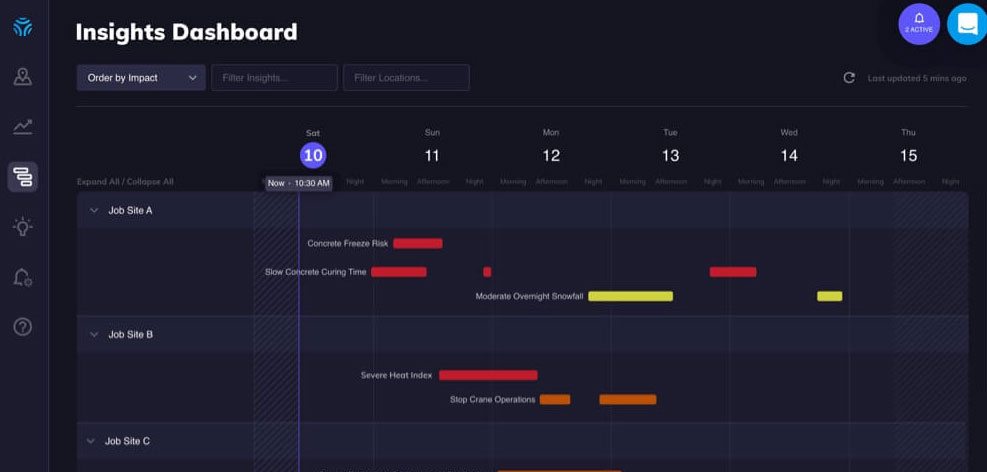
\includegraphics[width=\textwidth]{figs/climacell.jpg}
	\label{f.darksky-calendar}
	\legend{\small Fonte: \cite{dashboard-climacell}.}
\end{figure}

\subsection{Dark Sky}
\label{ss.darksky}
O Dark Sky é uma aplicação para simulação pluviométrica que foi comprada pela Apple em 2020. Uma de suas funcionalidades, apelidada de \emph{Time Machine} (Máquina do Tempo), consegue simular dados para mais de 15 anos no futuro.

Além disso, o Dark Sky oferece informações meteorológicas hiperlocais, com previsões minuto a minuto para entregar ao usuário informações exatas de quando a chuva vai começar ou acabar.

\begin{figure}[H]
	\caption{\small Função \emph{Time Machine} da aplicação Dark Sky.}
	\centering
	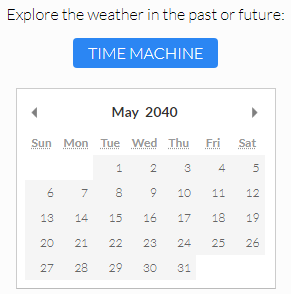
\includegraphics[scale=0.75]{figs/darkskyCalendar.PNG}
	\label{f.darksky-calendar}
	\legend{\small Fonte: \cite{darksky-main}.}
\end{figure}

\subsection{WeatherTAB}
\label{ss.weathertab}
Essa aplicação fornece um serviço de simulação da previsão de tempo há mais de cinquenta anos. Inicialmente o serviço era pago, mas recentemente a empresa decidiu abrir as portas ao público disponibilizando gratuitamente as suas previsões, que são financiadas por meio de publicidade.

O WeatherTAB fornece previsões meteorológicas com até 18 meses de antecedência, sem perda de precisão, segundo a própria organização \cite{weathertab}. Essas previsões são projetadas para ajudar no planejamento de atividades ao ar livre e indicam, com meses de antecedência, as datas em que há pouco ou muito risco de chuva ou neve.

\begin{figure}[H]
	\caption{\small Função de Previsão a Longo Prazo da aplicação WeatherTAB.}
	\centering
	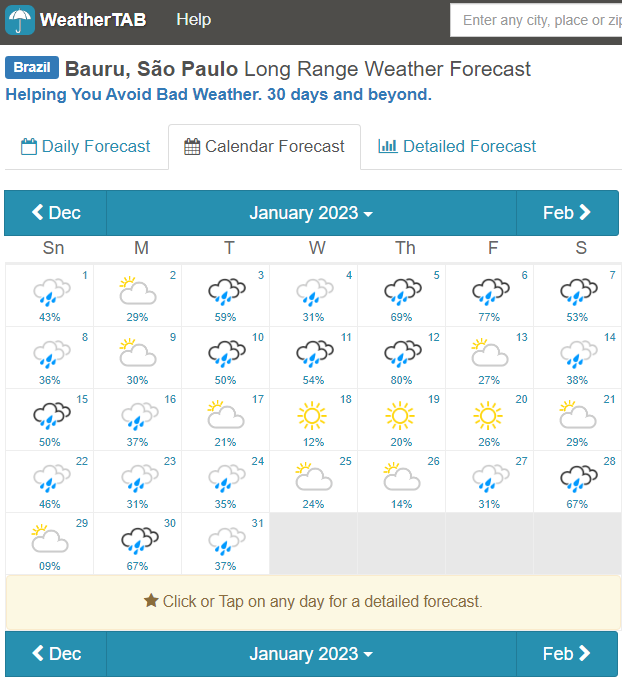
\includegraphics[scale=0.75]{figs/wtab-forecast.png}
	\label{f.darksky-calendar}
	\legend{\small Fonte: \cite{weathertab}.}
\end{figure}